\documentclass[paper=letter,11pt]{scrartcl}

\KOMAoptions{headinclude=true, footinclude=false}
\KOMAoptions{DIV=14, BCOR=5mm}
\KOMAoptions{numbers=noendperiod}
\KOMAoptions{parskip=half}
\addtokomafont{disposition}{\rmfamily}
\addtokomafont{part}{\LARGE}
\addtokomafont{descriptionlabel}{\rmfamily}
%\setkomafont{pageheadfoot}{\normalsize\sffamily}
\setkomafont{pagehead}{\normalsize\rmfamily}
%\setkomafont{publishers}{\normalsize\rmfamily}
\setkomafont{caption}{\normalfont\small}
\setcapindent{0pt}
\deffootnote[1em]{1em}{1em}{\textsuperscript{\thefootnotemark}\ }


\usepackage{amsmath}
\usepackage[varg]{txfonts}
\usepackage[T1]{fontenc}
\usepackage{graphicx}
\usepackage{xcolor}
\usepackage[american]{babel}
% hyperref is needed in many places, so include it here
\usepackage{hyperref}

\usepackage{xspace}
\usepackage{multirow}
\usepackage{float}


\usepackage{braket}
\usepackage{bbm}
\usepackage{relsize}
\usepackage{tcolorbox}

\def\ketY{\ensuremath{\ket {\Psi}}}
\def\iGeV{\ensuremath{\textrm{GeV}^{-1}}}
%\def\mp{\ensuremath{m_{\textrm{proton}}}}
\def\rp{\ensuremath{r_{\textrm{proton}}}}
\def\me{\ensuremath{m_{\textrm{electron}}}}
\def\aG{\ensuremath{\alpha_G}}
\def\rAtom{\ensuremath{r_{\textrm{atom}}}}
\def\rNucl{\ensuremath{r_{\textrm{nucleus}}}}
\def\GN{\ensuremath{\textrm{G}_\textrm{N}}}
\def\ketX{\ensuremath{\ket{\vec{x}}}}
\def\ve{\ensuremath{\vec{\epsilon}}}


\def\ABCDMatrix{\ensuremath{\begin{pmatrix} A &  B  \\ C  & D \end{pmatrix}}}
\def\xyprime{\ensuremath{\begin{pmatrix} x' \\ y' \end{pmatrix}}}
\def\xyprimeT{\ensuremath{\begin{pmatrix} x' &  y' \end{pmatrix}}}
\def\xy{\ensuremath{\begin{pmatrix} x \\ y \end{pmatrix}}}
\def\xyT{\ensuremath{\begin{pmatrix} x & y \end{pmatrix}}}

\def\IMatrix{\ensuremath{\begin{pmatrix} 0 &  1  \\ -1  & 0 \end{pmatrix}}}
\def\IBoostMatrix{\ensuremath{\begin{pmatrix} 0 &  1  \\ 1  & 0 \end{pmatrix}}}
\def\JThree{\ensuremath{\begin{pmatrix}    0 & -i & 0  \\ i & 0  & 0 \\ 0 & 0 & 0 \end{pmatrix}}} 
\def\JTwo{\ensuremath{\begin{bmatrix}    0 & 0 & -i  \\ 0 & 0  & 0 \\ i & 0 & 0 \end{bmatrix}}}
\def\JOne{\ensuremath{\begin{bmatrix}    0 & 0 & 0  \\ 0 & 0  & -i \\ 0 & i & 0 \end{bmatrix}}}
\def\etamn{\ensuremath{\eta_{\mu\nu}}}
\def\Lmn{\ensuremath{\Lambda^\mu_\nu}}
\def\dmn{\ensuremath{\delta^\mu_\nu}}
\def\wmn{\ensuremath{\omega^\mu_\nu}}
\def\be{\begin{equation*}}
\def\ee{\end{equation*}}
\def\bea{\begin{eqnarray*}}
\def\eea{\end{eqnarray*}}
\def\bi{\begin{itemize}}
\def\ei{\end{itemize}}
\def\fmn{\ensuremath{F_{\mu\nu}}}
\def\fMN{\ensuremath{F^{\mu\nu}}}
\def\bc{\begin{center}}
\def\ec{\end{center}}
\def\nus{$\nu$s}

\def\adagger{\ensuremath{a_{p\sigma}^\dagger}}
\def\lineacross{\noindent\rule{\textwidth}{1pt}}

\newcommand{\multiline}[1] {
\begin{tabular} {|l}
#1
\end{tabular}
}

\newcommand{\multilineNoLine}[1] {
\begin{tabular} {l}
#1
\end{tabular}
}



\newcommand{\lineTwo}[2] {
\begin{tabular} {|l}
#1 \\
#2
\end{tabular}
}

\newcommand{\rmt}[1] {
\textrm{#1}
}


%
% Units
%
\def\m{\ensuremath{\rmt{m}}}
\def\GeV{\ensuremath{\rmt{GeV}}}
\def\pt{\ensuremath{p_\rmt{T}}}


\def\parity{\ensuremath{\mathcal{P}}}

\usepackage{cancel}
\usepackage{ mathrsfs }
\def\bigL{\ensuremath{\mathscr{L}}}

\usepackage{ dsfont }



\usepackage{fancyhdr}
\fancyhf{}


\lhead{\Large 33-444} % \hfill Introduction to Particle Physics \hfill Spring 2020}
\chead{\Large Introduction to Particle Physics} % \hfill Spring 2020}
\rhead{\Large Spring 2020} % \hfill Introduction to Particle Physics \hfill Spring 2020}

\begin{document}
\thispagestyle{fancy}

\begin{center}
{\huge \textbf{Lecture 15}}
\end{center}

{\fontsize{14}{16}\selectfont

\textbf{\underline{From Last time...}} 

 
\underline{Example of scattering of 2 electrons}

\be
\ket{i} = \ket{e_1, e_2} \hspace*{1in}  \ket{f} = \ket{e_3, e_4}
\ee


\be
T_{fi} = V_{fi} + \sum_n V_{fn} \frac{1}{E_i-E_n} V_{ni} + ...
\ee

\bi
\item[-] $E_i$- is the initial (= final) energy
\item[-] $E_n$ - is the energy of the intermediate state
\ei

Now, the $\sum_n$ runs over energy thing in the Hilbert (Fock) space, however only certain states will be non-0.

In relativistic theory, the action-at-a-distance of EM is replaced by a process where 2 electrons interact with a $\gamma$ which travels at c. 
(This tells us there should be $\gamma$ in the intermediate state)
\be
V \sim e \int d^3x \psi \phi \psi  \hspace*{0.3in} \textrm{(Ignoring spin)}
\ee
this operator will have terms that go like ($\sim a_{e_3}^\dagger\ a_{\gamma}^\dagger\ a_{e_1}$)


However, here all terms involve $a_{\gamma}^\dagger$.\\
Because $\ket{i}$ and $\ket{f}$ do not contain a $\gamma$, $  V_{fi} = 0$

to get a non-zero term, we need $\ket{n}$ with a photon. 
\begin{figure}[h]
\centering
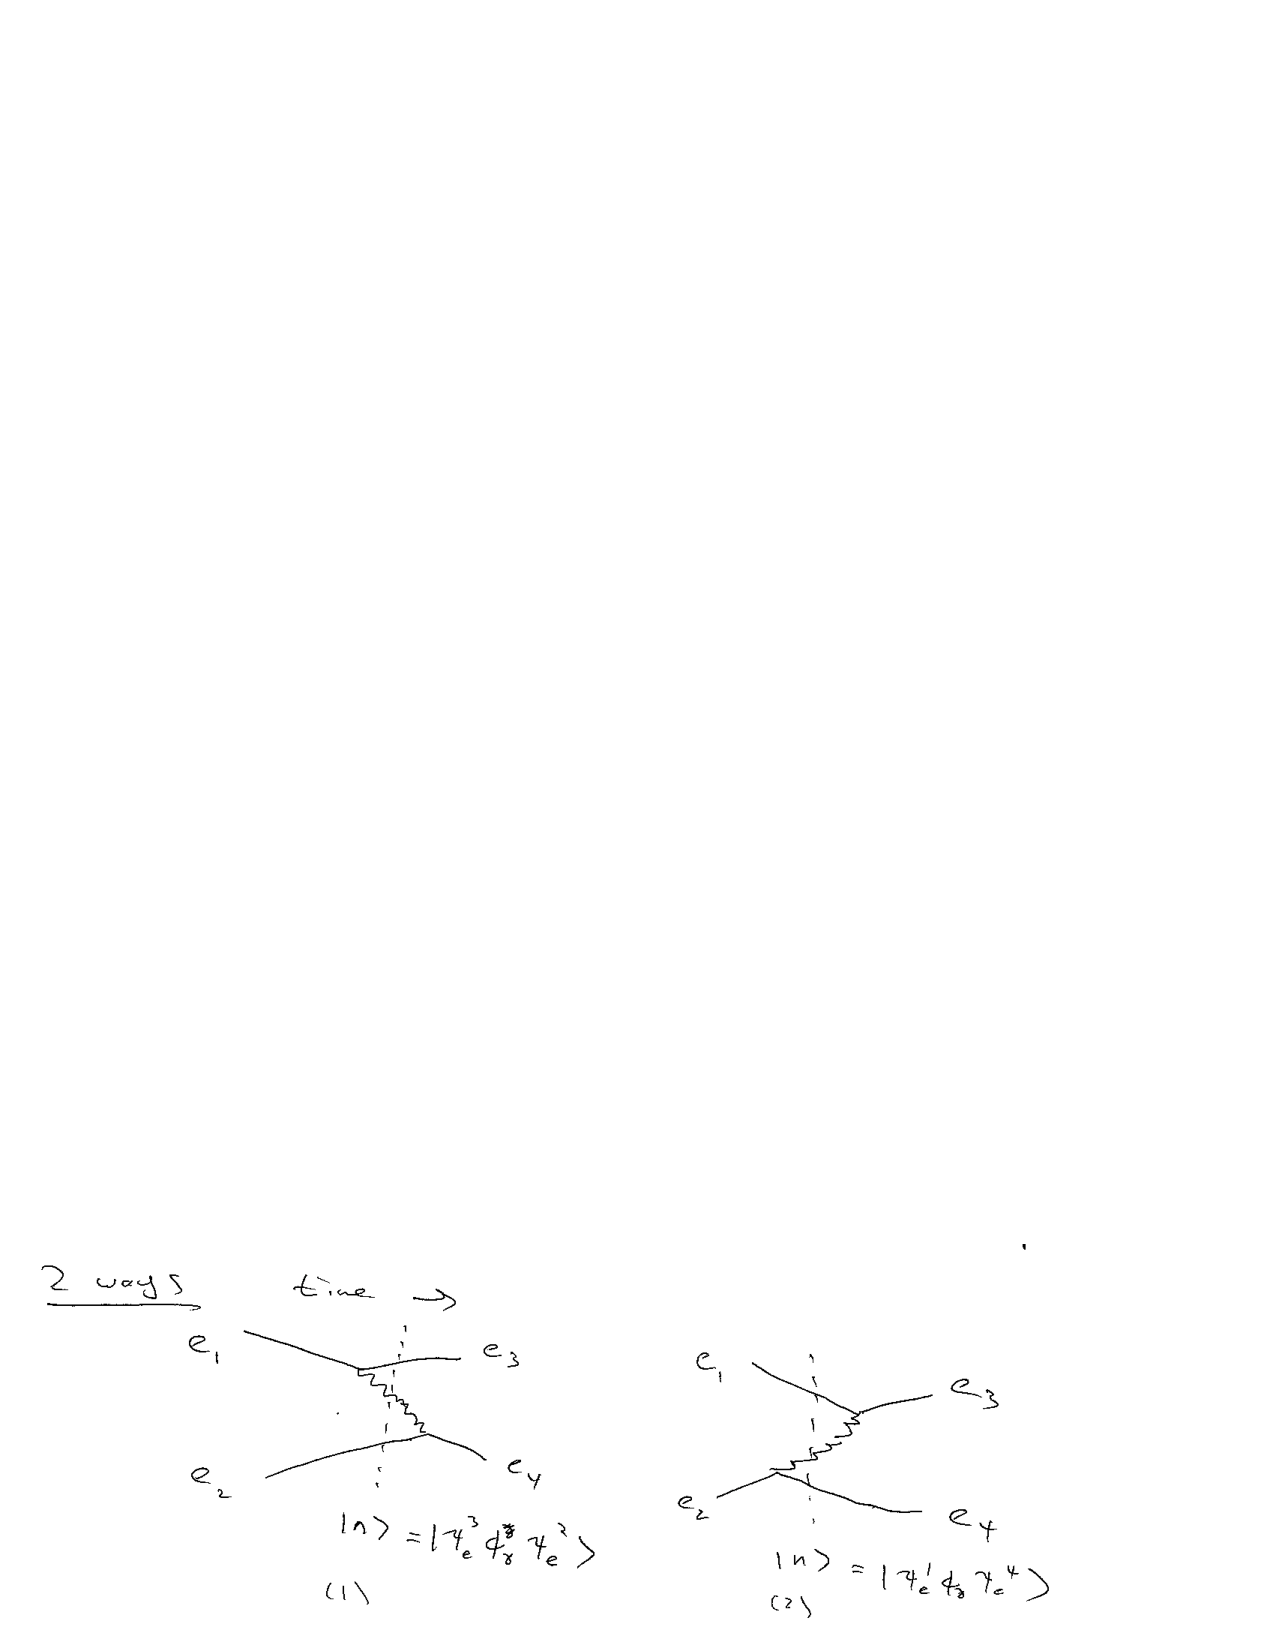
\includegraphics[width=0.99\textwidth]{./eeScattering.pdf}
\end{figure}



\be
T_{fi} = \frac{\braket{e_3 e_4|V|e_3 \gamma e_2}\braket{e_3 \gamma e_2|V|e_1 e_2 }}{(E_1+E_2) - (E_3 + E_4 + E_\gamma)} + \textrm{(2nd term)}
\ee
Note: $E_n \ne E_i$ which is allowed by uncertainty principle.


Look at 
\be
\braket{e_3 \gamma e_2|V|e_1 e_2} = \braket{\gamma e_3 |V|e_1}
\ee
(up to overall normalization from $\braket{e_2|e_2}$.

\fbox{\begin{minipage}{0.4\textwidth}
\be
\braket{\gamma|\phi_\gamma(x)|0} = e^{-ip_\gamma \cdot x}
\ee
\end{minipage}}


\bea
\braket{\gamma e_3|V|e_1} &=& e \int d^3x \braket{\gamma e_3|\psi_e \phi_\gamma \psi_e|e_1 }\\
&=& e \int d^3x e^{-i(p_3 + p_\gamma - p_1)x} = e (2\pi)^3 \delta(p_3 + p_\gamma - p_1)
\eea

Other product

\be
\braket{e_4|V|\gamma e_2} = e (2\pi)^3 \delta(p_4 -  p_\gamma - p_2)
\ee

Combining this gives
\be
T_{fi}^1 \sim \int d^3 p_\gamma\  \delta \delta  \frac{e^2 }{E_i - E_n}
\ee
where $E_i = (E_1 + E_2)$ and $E_n = (E_3 + E_2 + E_\gamma)$.


\be
T_{fi}^1 \sim   \frac{e^2 }{(E_1+E_2) - (E_3+E_2+E_\gamma)} = \frac{e^2 }{(E_1-E_3) - E_\gamma}
\ee

Same logic for 2nd term leads to
\be
T_{fi}^2 \sim  \frac{e^2 }{(E_2-E_4) - E_\gamma}
\ee


End of the day, need to add the two processes.


\fbox{\begin{minipage}{0.4\textwidth}
Note:
\be 
E_1+E_2 = E_3 + E_4
\ee
\be 
E_1-E_3 = E_4 - E_2 \equiv \Delta E
\ee
\end{minipage}}


\be
T^{1} + T^{2} = \frac{e^2}{\Delta E - E_\gamma} + \frac{e^2}{-\Delta E - E_\gamma} = \frac{2e^2 E_\gamma}{(\Delta E)^2 - E_\gamma^2}
\ee

define $k^\mu \equiv p_3^\mu - p_1^\mu = (\Delta E, \vec{p_\gamma})$

Note $k^\mu$ is not the photon momentum!  $k^2 \ne 0  (= (\Delta E)^2 - E_\gamma^2)$

\be
T_{fi} = \underbrace{2E_\gamma}_{\textrm{Related to normalization}} \frac{e^2}{k^2}
\ee

\underline{Summary} Standard ``old-fashion'' perturbation theory
\bi
\item[-] All states are physical (on-shell)
\item[-] Matrix element $V_{ij}$ vanishes unless 3-momentum conserved
\item[-] Energy \underline{not} conserved at each vertex
\item[-] Add all time orderings
\ei


Modern way to interpret same thing ``Feynam rules'' 

\underline{Summary} Feynman Rules
\bi
\item[-] Draw diagrams ignoring time ordering
\item[-] Vertices come from interactions in Lagrangian: factor of $i$ times coupling constant
\item[-] Internal lines get ``propagators'' $= \frac{i}{p^2 - m^2}$
\item[-] Lines connected to external points do not get propagators (scalars $\times$ 1 / spinors $\times$ u or v / spin-1 $\times \epsilon$)
\item[-] Four momenta is conserved at each vertex
\item[-] Integrate over all undetermined 4-momenta
\ei

\lineacross

\underline{Other Spins}

Scalar:
\be
\Phi (\vec{x}) = \int \cancel{d}^3p\ a^\dagger e^{-i p x} + b e^{+i p x}
\ee


Spin-1:
\be
A^\mu (\vec{x}) = \int \cancel{d}^3p\ a^\dagger_\gamma \epsilon^\mu e^{-i p x} + a_\gamma \epsilon^\mu e^{+i p x}
\ee
where, $\epsilon^\mu$ is the photon polarization vector, the solution for the Spin-1 relativistic equation of motion (ie: Maxwell's equations).
Here, we are taking the spin-1 particles to be thier own anti-particles (as is true for photons).


Spin-1/2:
\be
\Psi^\mu (\vec{x}) = \int \cancel{d}^3p\ a^\dagger v(p) e^{-i p x} + b u(p) e^{+i p x}
\ee
where, $u(p)$ and $v(p)$ are the dirac spinors, the solution for the Spin-1/2 relativistic equation of motion (ie: the dirac equation).


%
%Example: 
%
%\be
%L = -\frac{1}{2} (\partial_\mu \phi \partial^\mu \phi)^2 - \frac{1}{2}m^2 \phi^2 + \frac{g}{3!}\phi^3
%\ee
%
%Consider cross-section for $\phi\phi\rightarrow\phi\phi$ scattering.
%
%\be
%d\sigma = \frac{1}{(2E_1)(2E_2)|v_1-v_2|} |M|^2 d\Pi_{LIPS}
%\ee
%
%$p_1 + p_2 \rightarrow p_3 + p_4$
%
%
%In COM frame,  $\vec{p}_1 = -\vec{p}_2$ and $\vec{p}_3 = -\vec{p}_4$\\
%Also, $E_1 + E_2 = E_3+E_4 = E_{CM}$
%
%\be
%d\Pi_{LIPS} = (2\pi)^4 \delta^4(\sum p) \frac{d^3p_3}{(2\pi)^3} \frac{1}{2E_3} \frac{d^3p_4}{(2\pi)^3} \frac{1}{2E_4}
%\ee
%(integrating over $\vec{p}_4$)
%
%\be
%= \frac{1}{16\pi^2} d\Omega \int dp_f \frac{p_f^2}{E_3} \frac{1}{E_4} \delta(E_3+E_4-E_{CM})
%\ee
%where $p_f = |\vec{p}_3| = |\vec{p}_4|$ , $E_3 = \sqrt{m^2 + p_f^2}$, and $\int d^3p_f = \int dp_f p_f^2 d\Omega$
%
%Now change variables, 
%
%$p_f \rightarrow x = E_3 + E_4 - E_{CM}$
%
%\be
%dx = \frac{d}{dp_f}(E_3 + E_4 - E_{CM}) dp_f = \frac{p_f}{E_3} + \frac{p_f}{E_4}  = \frac{E_3 + E_4}{E_3E_4} p_f dp_f
%\ee
%
%$\Rightarrow$
%\be
%\frac{dp_f p_f^2}{E_3E_4} = \frac{dx p_f}{ E_{CM}}
%\ee
%
%
%\bea
%d\Pi_{LIPS} &=& \frac{1}{16\pi^2} d\Omega \int_{m_3+m_4-E_{CM}}^{\infty} dx \frac{p_f}{ E_{CM}} \delta(x) \\ 
%&=& \frac{1}{16\pi^2} d\Omega \frac{p_f}{ E_{CM}} \textrm{if $E_{CM} > m_3 + m_4$ else 0 }
%\eea
%
%\be
%d\sigma = \frac{1}{(2E_1)(2E_2)|v_1 - v_2|} \frac{1}{16\pi^2}d\Omega \frac{p_f}{ E_{CM}} |M|^2
%\ee
%
%\be
%|v_1 - v_2| = \left| \frac{|\vec{p}_1|}{E_1}  + \frac{|\vec{p}_2|}{E_2} \right| = p_i \frac{E_{CM}}{E_1 E_2}
%\ee
}
\end{document}

